%% 
%% Copyright 2019-2024 Elsevier Ltd
%% 
%% Version 2.4
%% 
%% This file is part of the 'CAS Bundle'.
%% --------------------------------------
%% 
%% It may be distributed under the conditions of the LaTeX Project Public
%% License, either version 1.2 of this license or (at your option) any
%% later version.  The latest version of this license is in
%%    http://www.latex-project.org/lppl.txt
%% and version 1.2 or later is part of all distributions of LaTeX
%% version 1999/12/01 or later.
%% 
%% The list of all files belonging to the 'CAS Bundle' is
%% given in the file `manifest.txt'.
%% 
%% Template article for cas-dc documentclass for 
%% double column output.

%\documentclass[a4paper,fleqn,longmktitle]{cas-dc}
\documentclass[a4paper,fleqn]{cas-dc}

%\usepackage[authoryear,longnamesfirst]{natbib}
%\usepackage[authoryear]{natbib}
\usepackage[numbers]{natbib}

\usepackage[utf8]{inputenc}
\usepackage[T1]{fontenc}

\usepackage[normalem]{ulem}
\usepackage{cancel}
\usepackage[most]{tcolorbox}

\usepackage[numbers]{natbib}
\usepackage{algorithm}

\usetikzlibrary{backgrounds, arrows.meta, positioning, fit} % Add any others you might need here

\usepackage{soul}
\usepackage{amsmath,amssymb,amsfonts}
\usepackage{amsthm} % 定理环境
\usepackage{mathrsfs}
\usepackage{graphicx}
\usepackage{multirow}
\usepackage{booktabs}
\usepackage{array}
\usepackage{tabularx}
\usepackage{makecell}
\usepackage{threeparttable}
\usepackage{varwidth}
\usepackage{caption}
\usepackage{calc}
\usepackage{url}
\usepackage{cleveref}
\usepackage{hyperref} 
\usepackage{listings}
\usepackage{algorithmicx}
\usepackage{algpseudocode}
\usepackage{seqsplit}
\usepackage{tabto}
\usepackage{textcomp}
\usepackage{manyfoot}
\usepackage[title]{appendix}
\usepackage{xcolor} % 统一在这里加载，移除后面的重复
\usepackage{tcolorbox} % 统一在这里加载
\tcbuselibrary{skins}
\usepackage[table]{xcolor}
\usepackage{changepage}

\usepackage{microtype}

\newtheorem{proposition}{Proposition}
\newtheorem{corollary}{Corollary}
\newtheorem{definition}{Definition}
\newtheorem{assumption}{Assumption}

\usepackage{enumitem}

\captionsetup[figure]{justification=justified, singlelinecheck=false}

% % 语言和字体
% \usepackage[english]{babel} % 有bug，该包不可引入
\usepackage[normalem]{ulem}
\usepackage{lipsum}
% % \usepackage{orcidlink}
% % \usepackage{orcidid}
\usepackage{ragged2e}


\usepackage{hyperref}
\usepackage{cleveref}

\usepackage{tikz}
\usetikzlibrary{
    shapes.geometric, % 用于菱形 (diamond)
    arrows.meta,      % 用于箭头样式 (stealth)
    positioning,      % 用于更精准的节点定位 (below left of 等)
    calc              % 用于坐标计算
}

% 定义你的自定义命令和环境（放在宏包之后）
\newtcolorbox{promptbox}[1][]{%
    title=Prompt Template,
    colframe=gray!50!black,
    colback=gray!10,
    fonttitle=\bfseries,
    boxsep=4pt,
    left=8pt, right=8pt,
    top=6pt, bottom=6pt,
    arc=2pt,
    fontupper=\small,
    boxrule=0.6pt,
    #1
}

\definecolor{mybgcolor}{HTML}{F4F4F4}

\tcbset{
    myshadowbox/.style={
        enhanced,
        skin=enhanced jigsaw, % 可选：更干净的渲染
        colback=mybgcolor,
        colframe=black,
        boxrule=0.5pt,
        arc=4pt,
        left=6pt, right=6pt, top=6pt, bottom=6pt,
        drop shadow=black!20 % 简洁、安全、有效
    }
}

\definecolor{mybgcolor}{HTML}{F4F4F4}
\tcbset{
    myshadowbox/.style={
        enhanced,
        skin=enhanced jigsaw,
        colback=mybgcolor,
        colframe=black,
        boxrule=0.5pt,
        arc=4pt,
        left=6pt, right=6pt, top=6pt, bottom=6pt,
        drop shadow=black!20
    }
}

\newcommand{\colorcell}[1]{
  \ifdim#1pt=0pt
    \cellcolor{orange!2}#1
  \else\ifdim#1pt<10pt
    \cellcolor{orange!10}#1
  \else\ifdim#1pt<20pt
    \cellcolor{orange!20}#1
  \else\ifdim#1pt<26pt
    \cellcolor{orange!26}#1
  \else\ifdim#1pt<29pt
    \cellcolor{orange!29}#1
  \else\ifdim#1pt<40pt
    \cellcolor{orange!40}#1
  \else\ifdim#1pt<50pt
    \cellcolor{orange!50}#1
  \else\ifdim#1pt<55pt
    \cellcolor{orange!55}#1
  \else\ifdim#1pt<60pt
    \cellcolor{orange!60}#1
  \else
    \cellcolor{orange!70}#1
  \fi\fi\fi\fi\fi\fi\fi\fi\fi
}

\newcommand{\vn}[1]{\text{#1}}

\newcommand{\orcid}[1]{\href{https://orcid.org/#1}{\includegraphics[height=0.8em]{0.ORCID-iD_icon_vector.pdf}}}

\newcommand{\sysname}{SoC\texttt{-}RCA}

%%%Author definitions
\def\tsc#1{\csdef{#1}{\textsc{\lowercase{#1}}\xspace}}
\tsc{WGM}
\tsc{QE}
\tsc{EP}
\tsc{PMS}
\tsc{BEC}
\tsc{DE}
%%%

\immediate\write18{texcount -inc -sum ADS-KGRCA-dc.tex > wordcount.txt}

\begin{document}
\let\WriteBookmarks\relax
\def\floatpagepagefraction{1}
\def\textpagefraction{.001}
\shorttitle{SoC-RCA}
\shortauthors{Dianlin Wang et~al.}

\title [mode = title]{Signal-to-Cause: Uni-Modal Analysis, Multi-Modal Fusion, and Causal Adjudication for Root Cause Localization}                      

\author[1,2]{Dianlin Wang\orcid{0009-0008-3099-6204}}[type=editor,
                        auid=000,bioid=1,
                        orcid=0009-0008-3099-6204]
\ead{wangdianlin@nudt.edu.cn}
\credit{Writing – original draft, Visualization, Validation, Methodology, Investigation, Conceptualization}

\author[1,2]{Tun Li\orcid{0000-0001-7498-3909}}[orcid=0000-0001-7498-3909]
\credit{Writing – review \& editing, Conceptualization}

\author[1,2]{Shangwen Wang\orcid{0000-0003-1469-2063}}[orcid=0000-0003-1469-2063]
\credit{Writing – review \& editing, Validation}

\author[4]{Zhuo Zhang\orcid{0000-0003-3243-1019}}[orcid=0000-0003-3243-1019]
\credit{Writing – review \& editing, Validation}

\author[1,2]{Bo Lin\orcid{0000-0001-5905-4677}}[orcid=0000-0001-5905-4677]
\credit{Writing – review \& editing}

\author[3]{Yan Lei\orcid{0000-0003-4504-6806}}[orcid=0000-0003-4504-6806]
\credit{Writing – review \& editing}

\author[1,2]{Xiaoguang Mao\orcid{0000-0003-4204-7424}}[orcid=0000-0003-4204-7424]
\credit{Writing – review \& editing}

\affiliation[1]{organization={National University of Defense Technology, College of Computer Science and Technology},
                addressline={Deya Road}, 
                city={Changsha},
                postcode={410073}, 
                state={Hunan},
                country={China}}

\affiliation[2]{organization={National University of Defense Technology, Laboratory of Complex \& Critical Software Environment},
                addressline={Deya Road}, 
                city={Changsha},
                postcode={410073}, 
                state={Hunan},
                country={China}}

\affiliation[3]{organization={Chongqing University},
            addressline={Shazheng Street}, 
            city={Chongqing},
            postcode={400030}, 
            state={Chongqing Shi},
            country={China}}

\affiliation[4]{organization={Army Special Operations College, Department of Special Technologies},
            addressline={Chongxin Road}, 
            city={Guilin},
            postcode={541000}, 
            state={Guangxi},
            country={China}}

\begin{abstract}
Failure localization in microservice systems is challenging because faults propagate across services through complex dependency chains, producing conflicting evidence across heterogeneous telemetry modalities.
Existing LLM-enhanced frameworks transform multi-modal data into natural language for agent-based reasoning but rely on a single anomaly detection channel---typically univariate statistical methods---and thus fail to distinguish true root causes from \emph{correlation disruptions}, where inter-variable dependencies break while each individual metric remains within normal bounds.

We present \sysname{}, a dual-channel root cause analysis framework that addresses the fundamental conflict between univariate and multivariate anomaly detection through a principled, LLM-arbitrated resolution mechanism.
\sysname{} runs two independent RCA pipelines in parallel: (1) a \textbf{univariate channel} using CNN-based pattern classification and SPOT anomaly scoring, and (2) a \textbf{multivariate channel} using configurable deep anomaly detectors (TranAD, USAD, GDN, among seven supported methods) to capture cross-metric correlation disruptions.
Each channel drives its own causal random walk on the same PCMCI causal graph, producing independent root-cause rankings.
When rankings diverge, a structured conflict classifier categorizes the disagreement into three scenarios, and an LLM-based arbitrator synthesizes a unified diagnosis with explicit reasoning---delegating final adjudication to causal graph structure when evidence is genuinely ambiguous.
We further introduce enhanced anomaly description generation with severity grading, cross-metric correlation analysis, and causal propagation path injection, which enrich the knowledge supplied to downstream LLM agents.
Experiments on the GAIA benchmark demonstrate that \sysname{} improves Top-3 localization accuracy by \textbf{X.X\%} over single-channel baselines while producing significantly more interpretable root-cause reports.

\end{abstract}

\begin{graphicalabstract}
\centering
  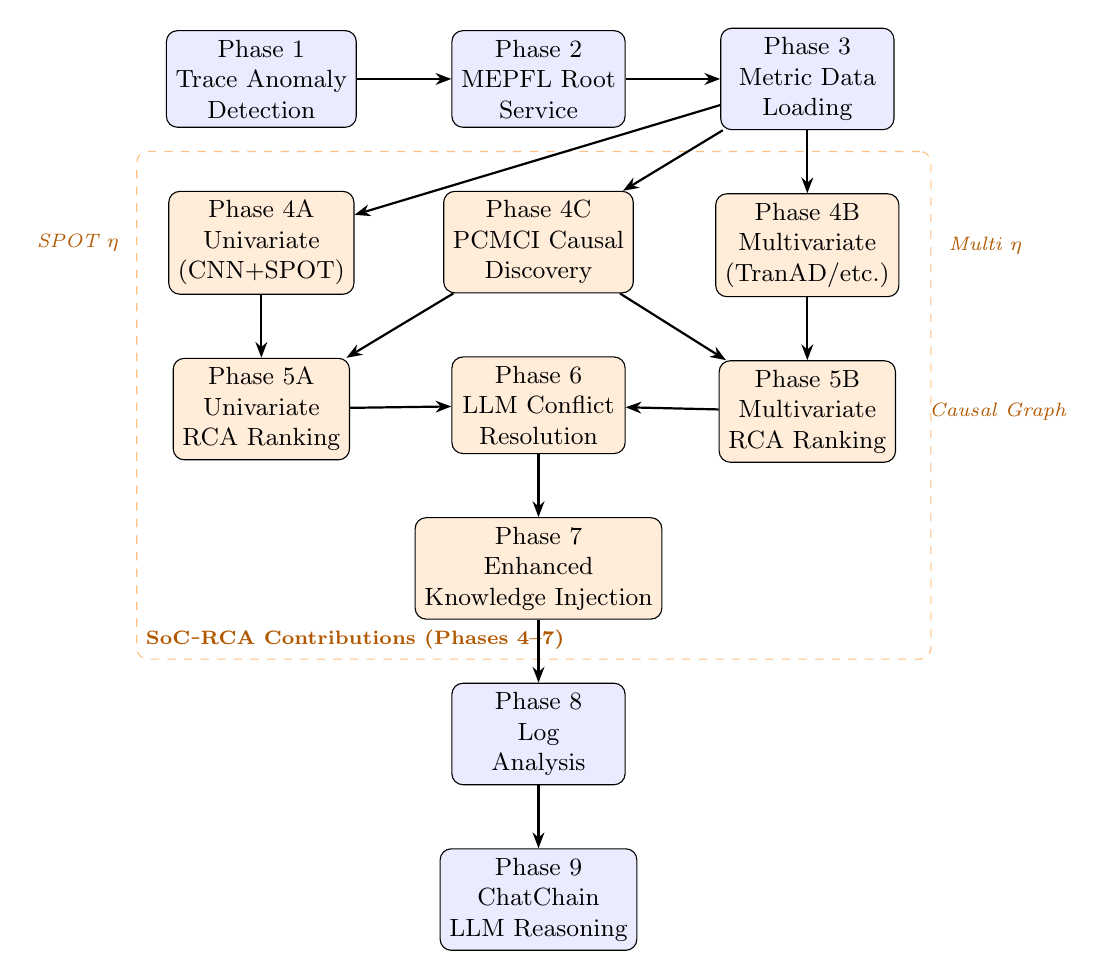
\begin{tikzpicture}[
    node distance=0.8cm and 1.2cm,
    phase/.style={draw, rounded corners, fill=blue!8, minimum width=2.2cm, minimum height=0.7cm, align=center, font=\small},
    newphase/.style={draw, rounded corners, fill=orange!15, minimum width=2.2cm, minimum height=0.7cm, align=center, font=\small},
    arrow/.style={-{Stealth[length=2mm]}, thick},
    dasharrow/.style={-{Stealth[length=2mm]}, thick, dashed},
  ]
    % Phases
    \node[phase] (p1) {Phase 1\\Trace Anomaly\\Detection};
    \node[phase, right=of p1] (p2) {Phase 2\\MEPFL Root\\Service};
    \node[phase, right=of p2] (p3) {Phase 3\\Metric Data\\Loading};

    % Phase 4: dual detection  拉大了垂直距离（从 0.8cm 改为 1.6cm）
    \node[newphase, below=of p1] (p4a) {Phase 4A\\Univariate\\(CNN+SPOT)};
    \node[newphase, below=of p3] (p4b) {Phase 4B\\Multivariate\\(TranAD/etc.)};
    \node[newphase, below=of p2] (p4c) {Phase 4C\\PCMCI Causal\\Discovery};

    % Phase 5: dual RCA
    \node[newphase, below=of p4a] (p5a) {Phase 5A\\Univariate\\RCA Ranking};
    \node[newphase, below=of p4b] (p5b) {Phase 5B\\Multivariate\\RCA Ranking};

    % Phase 6: conflict resolution
    \node[newphase, below=of p4c] (p6) {Phase 6\\LLM Conflict\\Resolution};

    % Phase 7: knowledge injection
    \node[newphase, below=of p6] (p7) {Phase 7\\Enhanced\\Knowledge Injection};

    % Phase 8-9
    \node[phase, below=of p7] (p8) {Phase 8\\Log\\Analysis};
    \node[phase, below=of p8] (p9) {Phase 9\\ChatChain\\LLM Reasoning};

    % Arrows
    \draw[arrow] (p1) -- (p2);
    \draw[arrow] (p2) -- (p3);
    \draw[arrow] (p3) -- (p4a);
    \draw[arrow] (p3) -- (p4b);
    \draw[arrow] (p3) -- (p4c);
    \draw[arrow] (p4a) -- (p5a);
    \draw[arrow] (p4b) -- (p5b);
    \draw[arrow] (p4c) -- (p5a);
    \draw[arrow] (p4c) -- (p5b);
    \draw[arrow] (p5a) -- (p6);
    \draw[arrow] (p5b) -- (p6);
    \draw[arrow] (p6) -- (p7);
    \draw[arrow] (p7) -- (p8);
    \draw[arrow] (p8) -- (p9);

    % Labels
    \node[left=0.5cm of p4a, font=\scriptsize\itshape, text=orange!70!black, align=right] {SPOT $\eta$};
    \node[right=0.5cm of p4b, font=\scriptsize\itshape, text=orange!70!black, align=left] {Multi $\eta$};
    \node[right=0.3cm of p5b, font=\scriptsize\itshape, text=orange!70!black] {Causal Graph};

    % Background group for new phases  标题左对齐，不再遮挡
    \begin{scope}[on background layer]
      \node[fit=(p4a)(p4b)(p4c)(p5a)(p5b)(p6)(p7),
            draw=orange!50, dashed, rounded corners, 
            inner sep=0.4cm,       % 左右边距（保持不动）
            inner ysep=0.5cm,      % 上下边距 → 改大这个，方框就纵向变长！
            label={[font=\scriptsize\bfseries, text=orange!70!black, anchor=south west]south west:\sysname{} Contributions (Phases 4--7)}] {};
    \end{scope}
  \end{tikzpicture}
\end{graphicalabstract}


\begin{highlights}
\item 11
\end{highlights}

\begin{keywords}
Root cause analysis \sep microservice failure localization \sep multi-modal anomaly detection \sep large language models \sep causal inference \sep conflict resolution
\end{keywords}


\maketitle

\section{Introduction}
\label{sec:intro}

Modern microservice architectures comprise tens to hundreds of loosely coupled services interconnected through complex dependency graphs.  When a failure occurs---whether resource exhaustion, a network partition, or a software defect---its effects \emph{cascade} across service boundaries, producing observable anomalies in multiple telemetry modalities simultaneously: metrics spike or shift, traces exhibit anomalous call patterns, and logs emit error messages~\cite{9213058,10.1145/3338906.3338961,10165686}.  Accurate and timely root cause analysis (RCA) is therefore critical for maintaining system reliability and minimizing business impact~\cite{10.1145/3715005}.

A distinguishing characteristic of microservice failures is that the majority---approximately 60\%---manifest as cascading cross-service effects that disrupt multiple metrics simultaneously, rather than as isolated single-point failures~\cite{10.1145/3542929.3563482}.  In such cascading failures, the fault may disrupt the \emph{inter-variable dependency structure}---the way metrics covary---while leaving each individual metric within its normal range.  This phenomenon, which we term \emph{correlation disruption}, poses a fundamental challenge for anomaly detection methods that examine metrics in isolation.

Recent advances in Large Language Models (LLMs) have opened a new paradigm for microservice failure localization: by transforming multi-modal telemetry data into structured natural language descriptions, LLM-based agents can perform interpretable root cause reasoning~\cite{11449471,10.1145/3627703.3629553,10.1145/3627673.3680016}.  However, existing LLM-enhanced frameworks employ \emph{single-channel} anomaly detection---typically univariate methods---which is blind to correlation disruptions and produces rankings biased toward metrics with the most extreme individual deviations.  Supplementing univariate detection with multivariate methods creates a further challenge: \emph{how to resolve conflicts when the two channels disagree}~\cite{DBLP:journals/pvldb/TuliCJ22,10.1145/3394486.3403392,deng2021graph}.  Moreover, ablation studies confirm that the anomaly description module---which supplies evidence to LLM agents---is the single most critical component for reasoning quality~\cite{11449471}.  Section~\ref{sec:background} provides a detailed analysis of these challenges.

We present \sysname{}, a dual-channel root cause analysis framework built on three key ideas.  \emph{First}, univariate and multivariate anomaly detection are complementary perspectives: the former excels at attributing extreme point anomalies to specific metrics, while the latter excels at detecting subtle correlation disruptions.  \sysname{} runs both channels in parallel, each driving its own causal random walk on a shared PCMCI causal graph to produce independent root-cause rankings.  \emph{Second}, when the two channels disagree, the resolution is delegated to causal reasoning---not heuristic rules---since the PCMCI graph encodes fault propagation paths and temporal ordering.  \emph{Third}, the evidence supplied to downstream LLM agents is enriched with severity grading, cross-metric correlation analysis, causal propagation paths, and explicit conflict resolution rationale.

This paper makes the following contributions:
\begin{enumerate}[leftmargin=*]
  \item A \textbf{dual-channel RCA architecture} where univariate (CNN+SPOT) and multivariate (configurable deep detectors) channels independently drive causal random walks on a shared PCMCI causal graph, producing independent root-cause rankings.

  \item An \textbf{LLM-arbitrated conflict resolution mechanism} that classifies disagreements into structured scenarios, invokes an LLM arbitrator for explicit reasoning, and delegates final adjudication to causal graph structure when evidence is genuinely ambiguous.

  \item \textbf{Enriched knowledge injection} with severity grading, cross-metric correlation analysis, causal propagation paths, and dual-channel concordance assessment, significantly enriching the evidence available to downstream LLM agents.

  \item A \textbf{comprehensive evaluation} on the GAIA benchmark demonstrating improvements in both localization accuracy and reasoning quality over single-channel baselines.
\end{enumerate}


\section{Background, Motivation, and Challenges}
\label{sec:background}

This section provides the foundational context for \sysname{}.  We first describe the telemetry data available in microservice systems and how faults propagate across services.  We then summarize the emerging paradigm of LLM-enhanced root cause analysis and identify the specific limitations that motivate our work.  Finally, we present a motivating example that illustrates why single-channel detection is insufficient and formalize the key challenges.

\subsection{Microservice Telemetry and Failure Propagation}

Modern microservice systems expose three complementary telemetry modalities for observability~\cite{9213058,10.1145/3338906.3338961,10165686}.  \textbf{Metrics} are time-series measurements of resource utilization and performance counters (e.g., CPU usage, memory consumption, request latency, error rate) collected at regular intervals.  \textbf{Traces} record the end-to-end path of individual requests across service boundaries, capturing call structures, dependencies, and per-span timing information.  \textbf{Logs} are semi-structured text entries emitted by services during execution, containing error messages, warnings, and diagnostic information.

Each modality captures a different facet of system behavior, and no single modality suffices for comprehensive fault diagnosis.  Metrics provide continuous numerical signals suitable for statistical anomaly detection, but lack the semantic context to explain \emph{why} a metric deviated.  Traces reveal the structural dependencies between services and can identify where latency accumulates, but provide limited insight into resource-level root causes.  Logs offer rich contextual and semantic information, but are noisy, voluminous, and difficult to aggregate systematically.

When a failure occurs in a microservice system, its effects propagate through the service dependency graph, often traversing multiple hops before becoming observable~\cite{10.1145/3715005}.  Empirical studies show that approximately 60\% of production incidents are multi-data correlated failures---cascading effects that disrupt multiple services and metrics simultaneously---rather than isolated single-point failures~\cite{10.1145/3542929.3563482}.  In such cascading failures, the fault may disrupt the \emph{inter-variable dependency structure}---the way metrics covary under normal operation---while leaving each individual metric within its historical normal range.  We refer to this phenomenon as \emph{correlation disruption} (formally defined in Definition~\ref{def:correlation}).

\subsection{LLM-Enhanced Root Cause Analysis}

A promising line of work has demonstrated that Large Language Models (LLMs) can serve as a reasoning substrate for failure localization~\cite{11449471,10.1145/3627703.3629553,10.1145/3627673.3680016}.  The key insight is that multi-modal telemetry data can be transformed into structured natural language descriptions, which LLM-based expert agents then analyze through multi-turn reasoning.  This paradigm offers two advantages over traditional numerical approaches: (1)~LLMs can integrate heterogeneous evidence from metrics, traces, and logs within a single reasoning chain, and (2)~the resulting diagnosis is expressed in natural language, providing the interpretability that on-call operators require.

The representative framework LocaleXpert~\cite{11449471} instantiates this paradigm through a multi-phase pipeline.  It processes traces via TraceAnomaly~\cite{9251058} for anomaly detection and MEPFL~\cite{10.1145/3338906.3338961} for root service localization.  For metrics, it employs a CNN-based pattern classifier that categorizes anomalies into 11 temporal patterns (e.g., spike, level shift, trend), combined with SPOT~\cite{10.1145/3097983.3098144} for per-metric anomaly scoring.  These anomaly scores feed into MicroCause, which constructs a PCMCI causal graph~\cite{9213058} and performs a temporal cause-oriented random walk to rank root cause metrics.  The anomaly descriptions, trace analyses, and log entries are then injected as knowledge into specialized LLM agents (Trace Expert, Metric Expert, Log Expert, Root Cause Expert), which collaborate through a ChatChain protocol to produce the final diagnosis.

A critical finding from the LocaleXpert ablation study is that the \emph{anomaly description module} is the single most important component for LLM reasoning quality.  Removing it (w/o AD) causes a 62\% drop in BLEU-4, a 52\% drop in G-sim, and a 10\% drop in W-rate on the GAIA benchmark~\cite{11449471}.  This confirms that the quality of the natural language evidence supplied to LLM agents directly determines diagnostic accuracy.

However, the existing framework relies on a \emph{single-channel} anomaly detection pipeline that uses only univariate methods (3-sigma) for metrics.  This design has two fundamental limitations:

\begin{enumerate}[leftmargin=*]
  \item \textbf{Correlation disruption blindness.}  Univariate methods examine each metric independently and cannot detect anomalies that arise from disrupted inter-variable dependencies.  When a cascading failure disrupts the correlation structure between metrics while each individual metric remains within its normal bounds, the system reports ``no anomaly detected'' despite an active failure.

  \item \textbf{Single-channel ranking bias.}  Even when univariate detection identifies anomalies, the resulting root-cause ranking is biased toward metrics exhibiting the most extreme individual deviations---which are often downstream symptoms rather than the true root cause.  Without a complementary perspective that considers the joint state of all metrics, the causal random walk may converge on a proximate but incorrect root cause.
\end{enumerate}

\subsection{Motivating Example}

To illustrate these limitations concretely, consider the following scenario drawn from a representative microservice system.  A database connection pool in service $s_{\text{db}}$ becomes exhausted due to a slow resource leak, reducing the number of available connections from 100 to 5 over a period of minutes.  As the pool depletes:

\begin{itemize}[leftmargin=*]
  \item The database latency ($s_{\text{db}}$\_latency) increases from 20ms to 35ms---a 1.5$\sigma$ deviation that remains within the 3-sigma threshold.
  \item The downstream service latency ($s_{\text{api}}$\_latency) increases from 50ms to 65ms---a 1.2$\sigma$ deviation, also within normal bounds.
  \item The connection pool utilization ($s_{\text{db}}$\_pool\_usage) rises from 60\% to 95\%---a 2$\sigma$ deviation, still within the 3-sigma threshold.
\end{itemize}

A univariate 3-sigma detector sees \emph{no anomaly} on any individual metric, because each deviation is too small to exceed the threshold.  The system produces an empty anomaly report, and the LLM agents receive no diagnostic evidence---a complete miss.

A multivariate detector, by contrast, observes that the \emph{joint behavior} of these three metrics has shifted: the previously stable ratio between database latency and API latency has changed, and the correlation between pool usage and latency has strengthened as the pool nears exhaustion.  The multivariate channel flags the system as anomalous and attributes the anomaly primarily to $s_{\text{db}}$\_pool\_usage and $s_{\text{db}}$\_latency.

Now consider a variant where the pool exhaustion triggers a secondary effect: a spike in error rate ($s_{\text{api}}$\_error\_rate) that exceeds the 3-sigma threshold.  The univariate channel correctly identifies the error rate spike but attributes the root cause to $s_{\text{api}}$ (where the spike is most extreme), while the multivariate channel correctly traces the anomaly origin to $s_{\text{db}}$ (where the correlation disruption began).  The two channels disagree on the root cause, requiring a principled resolution mechanism.

This example motivates both the dual-channel architecture (to capture what each channel misses) and the conflict resolution mechanism (to reconcile disagreements when both channels detect different aspects of the same failure).

\subsection{Key Challenges}

Based on the above analysis, we identify three challenges that a robust LLM-enhanced RCA framework must address:

\begin{enumerate}[leftmargin=*]
  \item \textbf{Challenge~1: Comprehensive anomaly detection.}  The framework must detect both point anomalies (captured by univariate methods) and correlation disruptions (captured by multivariate methods), since neither category alone covers the full spectrum of failure modes.  This requires running both detection channels in parallel and integrating their outputs.

  \item \textbf{Challenge~2: Principled conflict resolution.}  When the two detection channels disagree---one sees an anomaly while the other does not, or both see anomalies but attribute them to different root causes---the framework must resolve the conflict through a principled mechanism rather than a fixed priority rule.  The resolution must be explainable, enabling operators to understand \emph{why} one channel was trusted over another.

  \item \textbf{Challenge~3: Enriched evidence for LLM reasoning.}  The anomaly descriptions supplied to LLM agents must go beyond simple template filling to include statistical context, cross-metric correlations, causal propagation paths, and explicit conflict resolution rationale.  The LLM should understand not just \emph{what} was detected, but \emph{why} a particular diagnosis was reached.
\end{enumerate}

These three challenges map directly to the three core contributions of \sysname{}, which we describe in Section~\ref{sec:method}.



% ======================================================================
%  III. METHODOLOGY
% ======================================================================
\section{Methodology}
\label{sec:method}

\subsection{Problem Formulation and System Overview}

Consider a microservice system $\mathcal{S}$ comprising $M$ services $\{s_1, \ldots, s_M\}$, where each service $s_m$ exposes a set of performance metrics (e.g., CPU usage, memory consumption, response latency).  Let $\mathbf{X} \in \mathbb{R}^{T \times N}$ denote the multivariate time series of $N$ metrics observed over $T$ timesteps, where column $i$ corresponds to metric $x_i$.  Given a failure incident reported at time $t_f$, the goal of root cause analysis is to identify the metric (or set of metrics) that most likely initiated the observed anomalies.

We distinguish two categories of anomalies that complicate this task:
\begin{definition}[Point Anomaly]
A metric $x_i$ exhibits a point anomaly at time $t$ if its observed value $x_i(t)$ deviates significantly from its historical distribution $P(x_i)$, i.e., $x_i(t) \notin [\mu_i - k\sigma_i, \mu_i + k\sigma_i]$ for threshold $k$.
\end{definition}

\begin{definition}[Correlation Disruption]\label{def:correlation}
A set of metrics $\{x_{i_1}, \ldots, x_{i_p}\}$ exhibits a correlation disruption if their joint distribution $P(x_{i_1}, \ldots, x_{i_p})$ at time $t_f$ differs significantly from the normal joint distribution, even though each marginal distribution $P(x_{i_j})$ remains within normal bounds.
\end{definition}

Point anomalies are detectable by univariate methods operating on individual metrics.  Correlation disruptions, by contrast, require multivariate methods that model inter-variable dependencies.  Since approximately 60\% of microservice failures manifest as cascading effects that disrupt correlation structures~\cite{10.1145/3542929.3563482}, a robust RCA framework must address both categories.

Figure~\ref{fig:architecture} presents the overall architecture of \sysname{}.  Given a failure incident described by a natural language task prompt (e.g., ``At 2021/07/01 11:54 have exceptions in the microservice system''), the system executes a nine-phase pipeline:

\begin{enumerate}[leftmargin=*]
  \item \textbf{Trace Anomaly Detection}: Detects structural and temporal anomalies in distributed traces using TraceAnomaly~\cite{9251058}, generating natural language descriptions.
  \item \textbf{Trace Root Service Localization}: Uses MEPFL~\cite{10.1145/3338906.3338961} (Random Forest + MLP) to identify the top-5 root cause services from trace data.
  \item \textbf{Metric Data Loading}: Loads and preprocesses metric time-series data from the MicroCause input format.
  \item \textbf{Dual Anomaly Detection}: Runs univariate (CNN + SPOT) and multivariate (configurable deep detector) anomaly detection \emph{in parallel}, producing independent anomaly scores and feature rankings.
  \item \textbf{Dual-Channel Root Cause Analysis}: Each channel drives its own causal random walk on the shared PCMCI causal graph, producing independent root-cause metric rankings.
  \item \textbf{LLM Conflict Resolution}: Classifies the conflict scenario, invokes an LLM arbitrator, and produces a unified diagnosis with explicit reasoning.
  \item \textbf{Enhanced Knowledge Injection}: Injects enriched anomaly descriptions, causal propagation paths, cross-metric correlations, and concordance analysis into the LLM agent prompts.
  \item \textbf{Log Analysis}: The Log Expert agent analyzes raw log entries around the failure time window.
  \item \textbf{ChatChain LLM Reasoning}: Multi-agent collaboration (Trace Expert, Metric Expert, Log Expert, Root Cause Expert) produces the final interpretable diagnosis report.
\end{enumerate}

Phases 1--3 handle trace analysis and metric data loading; Phases 8--9 handle log analysis and multi-agent LLM reasoning.  These phases follow established approaches~\cite{9251058,10.1145/3338906.3338961,11449471}.  The core contributions of \sysname{} lie in Phases 4--7, which we describe in detail below.

\begin{figure*}[t]
  \centering
  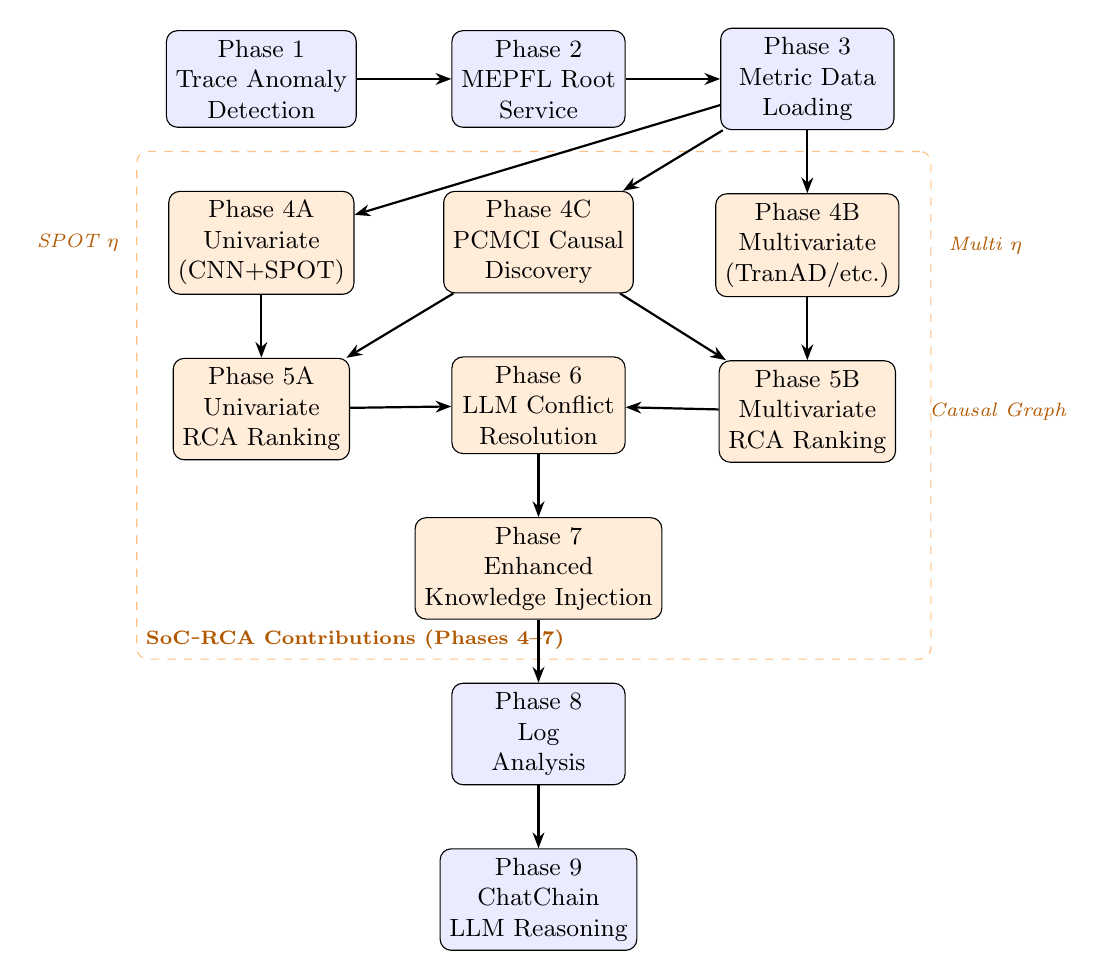
\begin{tikzpicture}[
    node distance=0.8cm and 1.2cm,
    phase/.style={draw, rounded corners, fill=blue!8, minimum width=2.2cm, minimum height=0.7cm, align=center, font=\small},
    newphase/.style={draw, rounded corners, fill=orange!15, minimum width=2.2cm, minimum height=0.7cm, align=center, font=\small},
    arrow/.style={-{Stealth[length=2mm]}, thick},
    dasharrow/.style={-{Stealth[length=2mm]}, thick, dashed},
  ]
    % Phases
    \node[phase] (p1) {Phase 1\\Trace Anomaly\\Detection};
    \node[phase, right=of p1] (p2) {Phase 2\\MEPFL Root\\Service};
    \node[phase, right=of p2] (p3) {Phase 3\\Metric Data\\Loading};

    % Phase 4: dual detection  拉大了垂直距离（从 0.8cm 改为 1.6cm）
    \node[newphase, below=of p1] (p4a) {Phase 4A\\Univariate\\(CNN+SPOT)};
    \node[newphase, below=of p3] (p4b) {Phase 4B\\Multivariate\\(TranAD/etc.)};
    \node[newphase, below=of p2] (p4c) {Phase 4C\\PCMCI Causal\\Discovery};

    % Phase 5: dual RCA
    \node[newphase, below=of p4a] (p5a) {Phase 5A\\Univariate\\RCA Ranking};
    \node[newphase, below=of p4b] (p5b) {Phase 5B\\Multivariate\\RCA Ranking};

    % Phase 6: conflict resolution
    \node[newphase, below=of p4c] (p6) {Phase 6\\LLM Conflict\\Resolution};

    % Phase 7: knowledge injection
    \node[newphase, below=of p6] (p7) {Phase 7\\Enhanced\\Knowledge Injection};

    % Phase 8-9
    \node[phase, below=of p7] (p8) {Phase 8\\Log\\Analysis};
    \node[phase, below=of p8] (p9) {Phase 9\\ChatChain\\LLM Reasoning};

    % Arrows
    \draw[arrow] (p1) -- (p2);
    \draw[arrow] (p2) -- (p3);
    \draw[arrow] (p3) -- (p4a);
    \draw[arrow] (p3) -- (p4b);
    \draw[arrow] (p3) -- (p4c);
    \draw[arrow] (p4a) -- (p5a);
    \draw[arrow] (p4b) -- (p5b);
    \draw[arrow] (p4c) -- (p5a);
    \draw[arrow] (p4c) -- (p5b);
    \draw[arrow] (p5a) -- (p6);
    \draw[arrow] (p5b) -- (p6);
    \draw[arrow] (p6) -- (p7);
    \draw[arrow] (p7) -- (p8);
    \draw[arrow] (p8) -- (p9);

    % Labels
    \node[left=0.5cm of p4a, font=\scriptsize\itshape, text=orange!70!black, align=right] {SPOT $\eta$};
    \node[right=0.5cm of p4b, font=\scriptsize\itshape, text=orange!70!black, align=left] {Multi $\eta$};
    \node[right=0.3cm of p5b, font=\scriptsize\itshape, text=orange!70!black] {Causal Graph};

    % Background group for new phases  标题左对齐，不再遮挡
    \begin{scope}[on background layer]
      \node[fit=(p4a)(p4b)(p4c)(p5a)(p5b)(p6)(p7),
            draw=orange!50, dashed, rounded corners, 
            inner sep=0.4cm,       % 左右边距（保持不动）
            inner ysep=0.5cm,      % 上下边距 → 改大这个，方框就纵向变长！
            label={[font=\scriptsize\bfseries, text=orange!70!black, anchor=south west]south west:\sysname{} Contributions (Phases 4--7)}] {};
    \end{scope}
  \end{tikzpicture}
  \caption{Architecture of \sysname{}.  Phases highlighted in orange (4--7) represent the key contributions: dual-channel anomaly detection and RCA, LLM-arbitrated conflict resolution, and enriched knowledge injection.  The shared PCMCI causal graph serves as the structural backbone for both RCA channels.}
  \label{fig:architecture}
\end{figure*}

\subsection{Dual-Channel Anomaly Detection}
\label{sec:dual_detection}

The fundamental premise of \sysname{} is that point anomalies and correlation disruptions provide complementary evidence for root cause analysis, and that neither alone is sufficient.  The univariate channel excels at identifying \emph{which specific metric} has deviated from its normal behavior, producing interpretable per-metric anomaly scores.  The multivariate channel excels at detecting \emph{whether the system as a whole} exhibits abnormal behavior, even when no individual metric is out of bounds.  By running both channels in parallel, \sysname{} ensures comprehensive anomaly coverage across the full spectrum of failure modes.

\paragraph{Univariate channel: CNN-based pattern classification and SPOT scoring.}
The univariate channel processes each metric independently through two complementary mechanisms.  First, a 1D-CNN classifier adapted for time-series analysis classifies detected anomalies into 11 patterns: single/double spike, single/double dip, level shift up/down, transient level shift up/down, steady increase/decrease, and fluctuations.  These patterns capture the distinctive temporal signatures of different failure modes---spikes indicate sudden transient events (e.g., a brief traffic burst), level shifts indicate sustained state changes (e.g., resource exhaustion), and trends indicate progressive degradation (e.g., a memory leak).  For each anomalous metric, the system generates a structured natural language description using pattern-specific templates that include temporal boundaries (start, end, duration), statistical features (mean, peak, $\sigma$-deviation, change magnitude), severity classification (mild/moderate/severe/critical based on $\sigma$-deviation), and cross-metric alerts when multiple metrics of the same service are simultaneously anomalous.

Second, the Streaming Percentile-based Outlier Test (SPOT/dSPOT)~\cite{10.1145/3097983.3098144} computes a per-metric anomaly deviation score $\eta_i$ for each metric $i$.  SPOT models the tail distribution of each metric using extreme value theory and identifies observations that exceed an automatically calibrated threshold, controlling the false positive rate at a user-specified significance level.  The resulting $\eta$ vector $\boldsymbol{\eta}^{\text{SPOT}} = (\eta_1, \ldots, \eta_N)$ serves as the prior anomaly signal for the univariate RCA channel.

\paragraph{Multivariate channel: deep reconstruction-based detection.}
The multivariate channel analyzes all metrics jointly to detect anomalies that arise from disrupted inter-variable dependencies.  The underlying principle is that deep generative models trained on normal data learn to reconstruct normal joint behavior accurately, but produce large reconstruction errors when the input exhibits abnormal correlation structures---even if each individual variable remains within its normal range.

\sysname{} supports seven deep learning methods through a unified factory interface: TranAD~\cite{DBLP:journals/pvldb/TuliCJ22} (dual-phase self-conditioning Transformer, default), USAD~\cite{10.1145/3394486.3403392} (dual autoencoder with adversarial training), OmniAnomaly~\cite{10.1145/3292500.3330672} (GRU-based VAE with planar normalizing flows), MAD-GAN~\cite{10.1007/978-3-030-30490-4_56}, MSCRED~\cite{10.1609/aaai.v33i01.33011409} (ConvLSTM encoder-decoder), GDN~\cite{deng2021graph} (graph attention network), and MTAD-GAT~\cite{10.1109/ICDM50108.2020.00093} (dual graph attention with GRU).  All detectors share a common \texttt{train}/\texttt{detect} interface: given normal training data, each model learns a reconstruction or prediction function; during detection, the per-timestep, per-feature reconstruction error $e_{t,i}$ quantifies how anomalous each metric is at each point in time.

The feature ranking provides a multivariate attribution: for each metric $i$, the total contribution is $c_i = \sum_{t} e_{t,i}$, where $e_{t,i}$ is the per-feature reconstruction error at timestep $t$.  This ranking is converted to a multivariate anomaly signal $\boldsymbol{\eta}^{\text{multi}}$ via magnitude-normalized scaling:
\begin{equation}
  \eta^{\text{multi}}_i = \frac{c_i}{\max_j c_j} \cdot \max_j \eta^{\text{SPOT}}_j
  \label{eq:multi_eta}
\end{equation}
This scaling ensures that $\boldsymbol{\eta}^{\text{multi}}$ has comparable magnitude to $\boldsymbol{\eta}^{\text{SPOT}}$, enabling both signals to be used interchangeably as priors for the causal random walk.  Intuitively, $\eta^{\text{multi}}_i$ measures how much metric $i$ contributes to the overall multivariate reconstruction error, normalized by the strongest univariate anomaly signal.


\subsection{Causal Graph Construction and Root Cause Analysis}
\label{sec:dual_rca}

Anomaly detection identifies \emph{what} is anomalous, but root cause analysis requires determining \emph{why}---distinguishing the initiating fault from its downstream symptoms.  \sysname{} addresses this by constructing a causal graph that encodes fault propagation paths and temporal ordering, then performing random walks to rank metrics by their likelihood of being the root cause.

\paragraph{PCMCI causal discovery.}
Both RCA channels share a single PCMCI causal graph~\cite{9213058}, constructed from the full metric time-series data.  PCMCI (PC algorithm with Momentary Conditional Independence) discovers time-lagged causal relationships through a two-stage procedure: the PC stage identifies candidate causal parents for each variable using conditional independence tests, and the MCI stage refines these links by testing momentary conditional independence---whether variable $x_j$ at lag $\tau$ has a direct effect on $x_i$ at time $t$, conditional on the estimated parents of both variables.  The result is a directed graph $\mathcal{G} = (\mathcal{V}, \mathcal{E})$ where $\mathcal{V}$ is the set of $N$ metric nodes and $\mathcal{E}$ is the set of causal edges, each annotated with a temporal delay $\tau$ and a strength measure (partial correlation).  Critically, this shared graph ensures that differences in root-cause rankings between the two channels arise \emph{solely} from the different anomaly priors ($\boldsymbol{\eta}^{\text{SPOT}}$ vs.\ $\boldsymbol{\eta}^{\text{multi}}$), not from different graph structures, enabling a controlled attribution of the impact of detection methodology.

\paragraph{Transition probability matrix.}
From the causal graph $\mathcal{G}$, the system constructs a transition probability matrix $Q \in \mathbb{R}^{N \times N}$ that encodes how likely a random walker is to transition from metric $i$ to metric $j$:
\begin{equation}
  Q_{ij} = \rho \cdot |r_{ij \cdot \mathcal{V} \setminus \{i,j\}}| + (1-\rho) \cdot \mathbb{1}[(i,j) \in \mathcal{E}]
  \label{eq:q_matrix}
\end{equation}
where $r_{ij \cdot \mathcal{V} \setminus \{i,j\}}$ is the partial correlation between metrics $i$ and $j$ controlling for all other metrics, $\mathbb{1}[(i,j) \in \mathcal{E}]$ indicates the presence of a causal edge, and $\rho \in [0,1]$ balances structural influence (the causal graph topology) against statistical influence (the correlation strength).  This design ensures that transitions follow causal paths but are weighted by the strength of statistical association, combining the complementary strengths of graph structure and data-driven evidence.

\paragraph{Dual-channel root cause scoring.}
A random walk of $S$ steps (default: 1000 walks, sampled every 15 steps) starting from the frontend service node produces a visitation count vector $\mathbf{v} = (v_1, \ldots, v_N)$, recording how often each metric node is visited.  Intuitively, metrics that are visited more frequently are more central in the causal propagation network and thus more likely to lie on the fault's propagation path.

Each channel computes a root cause score $\gamma_i$ for metric $i$ by combining the visitation frequency with its channel-specific anomaly prior:
\begin{equation}
  \gamma_i = \lambda \cdot \frac{v_i}{\sum_j v_j} + (1 - \lambda) \cdot \eta_i
  \label{eq:gamma}
\end{equation}
where $\lambda \in [0,1]$ balances causal graph structure ($v_i / \sum_j v_j$, the normalized visitation frequency) against anomaly evidence ($\eta_i$), and $\eta_i$ is either $\eta^{\text{SPOT}}_i$ (univariate channel) or $\eta^{\text{multi}}_i$ (multivariate channel).  The first term captures the \emph{topological} importance of metric $i$ in the causal propagation network; the second term captures the \emph{empirical} anomalousness of metric $i$ as detected by the corresponding channel.  By combining both signals, $\gamma_i$ ranks metrics that are both causally central and empirically anomalous higher than metrics that satisfy only one criterion.

The two channels produce independent rankings:
\begin{equation}
  \text{Rank}^{\text{uni}} = \text{argsort}(\boldsymbol{\gamma}^{\text{uni}}, \text{desc}), \quad
  \text{Rank}^{\text{multi}} = \text{argsort}(\boldsymbol{\gamma}^{\text{multi}}, \text{desc})
  \label{eq:ranking}
\end{equation}
Because both channels share the same $Q$-matrix and visitation counts $\mathbf{v}$, the only difference between $\text{Rank}^{\text{uni}}$ and $\text{Rank}^{\text{multi}}$ is the anomaly prior $\boldsymbol{\eta}$.  This controlled comparison isolates the impact of the detection method on root-cause attribution, making the subsequent conflict resolution principled rather than ad hoc.


\subsection{LLM-Arbitrated Conflict Resolution}
\label{sec:conflict}

When the univariate and multivariate channels produce different root-cause rankings, the system must resolve the disagreement.  A simple ensemble or fixed-priority rule would be inadequate because the optimal resolution strategy depends on the \emph{type} of conflict: a multivariate-only detection calls for trusting the multivariate channel, whereas a univariate-only detection may indicate noise or a genuine isolated fault.  \sysname{} addresses this by first classifying the conflict scenario, then applying a scenario-specific resolution strategy guided by a consistent principle: \emph{multivariate detection answers ``is the system anomalous?'', univariate detection answers ``which specific metric?'', and causal reasoning is the final arbiter}.

\paragraph{Conflict scenario classification.}
Given the dual-channel rankings and the detection-level anomaly flags ($\text{anomaly}^{\text{uni}}$, $\text{anomaly}^{\text{multi}}$), the system classifies the situation into one of four scenarios as shown in Table~\ref{tab:scenarios}.  The classification is based on two binary signals: whether each channel detects a system-level anomaly, and whether the top-$k$ root-cause rankings from the two channels overlap.  An overlap of $\geq 2$ metrics in the top-5 is considered agreement.

\begin{table}[h]
  \centering
  \caption{Conflict scenario classification and resolution strategy.}
  \label{tab:scenarios}
  \begin{tabular}{@{}p{0.12\linewidth}p{0.35\linewidth}p{0.40\linewidth}@{}}
    \toprule
    \textbf{Scenario} & \textbf{Observation} & \textbf{Strategy} \\
    \midrule
    Consistent & Both rankings agree ($\geq$2 top-5 overlap) & Merge descriptions; use agreed ranking \\
    S1 & Multi=anom, Uni=normal & Trust multivariate RCA (correlation disruption) \\
    S2 & Uni=anom, Multi=normal & Trust multivariate assessment; retain univariate as supplementary evidence \\
    S3 & Both=anom, different roots & Merge candidate sets; delegate to causal reasoning \\
    \bottomrule
  \end{tabular}
\end{table}

In Scenario~1 (correlation disruption), the univariate channel's silence is expected---by Definition~2, each metric individually is normal---so the multivariate ranking is trusted.  In Scenario~2 (isolated noise), the multivariate channel's normal verdict suggests the univariate alert is either noise or a non-critical fluctuation; the univariate evidence is retained as supplementary context but does not override the multivariate assessment.  In Scenario~3 (root cause divergence), both channels detect genuine anomalies but attribute them to different metrics, requiring a principled fusion mechanism.

\paragraph{LLM arbitration.}
For each conflict scenario, the system constructs a scenario-specific prompt that provides the LLM with the full evidence from both channels: anomaly flags, per-metric scores, pattern classifications, and the causal graph structure.  The LLM is asked to analyze the conflicting evidence and produce a structured response containing a consistency assessment, the trusted channel, a natural language anomaly summary, merged root cause candidates, step-by-step reasoning, and a correlation disruption analysis.  The LLM's role is not to override the detection results, but to synthesize a coherent narrative that explains \emph{why} one channel's evidence is more reliable in the current scenario, producing an interpretable diagnosis for downstream agents.

\paragraph{Causal re-arbitration for Scenario~3.}
When both channels detect anomalies but disagree on root cause (Scenario~3), simply picking one channel would discard valid evidence from the other.  Instead, \sysname{} fuses the evidence from both channels and delegates final adjudication to the causal graph through the following procedure:
\begin{enumerate}[leftmargin=*]
  \item \textbf{Merge} the candidate sets from both channels (up to 10 metrics).
  \item \textbf{Construct a boost vector} $\mathbf{b} \in \mathbb{R}^N$ that rewards metrics supported by both channels:
  \begin{equation}
    b_i = \begin{cases}
      2.0 & \text{if metric } i \text{ is in both channels' top-5} \\
      1.5 & \text{if metric } i \text{ is in one channel's top-5} \\
      1.0 & \text{otherwise}
    \end{cases}
  \end{equation}
  \item \textbf{Compute a blended anomaly prior}: $\boldsymbol{\eta}^{\text{blend}} = \frac{\boldsymbol{\eta}^{\text{SPOT}} + \boldsymbol{\eta}^{\text{multi}}}{2} \odot \mathbf{b}$, where $\odot$ denotes element-wise multiplication.
  \item \textbf{Re-run the causal random walk} with $\boldsymbol{\eta}^{\text{blend}}$ to produce the final arbitrated ranking.
\end{enumerate}
The boost vector design reflects a principled trade-off: metrics flagged by both channels receive the strongest amplification ($2.0\times$), reflecting high confidence from independent evidence sources; metrics flagged by only one channel receive moderate amplification ($1.5\times$), retaining their contribution while avoiding premature elimination.  The causal random walk then uses the graph topology and temporal ordering to determine which of the boosted metrics is the true root cause---an upstream metric in the causal chain will accumulate more visits than a downstream symptom, ensuring that the final ranking reflects causal rather than merely correlational evidence.


\subsection{Enriched Knowledge Injection for LLM Reasoning}
\label{sec:knowledge}

The preceding phases produce a rich set of intermediate results: per-metric anomaly scores, pattern classifications, multivariate reconstruction errors, causal graph edges, and conflict resolution rationale.  However, these results must be communicated to the downstream LLM agents (Phases 8--9) as natural language, and the quality of this communication directly determines reasoning quality.  Prior ablation studies~\cite{11449471} confirm that the anomaly description module is the single most critical component for LLM reasoning performance---removing it causes the steepest decline across all evaluation metrics.

\sysname{} enriches the evidence supplied to LLM agents along four complementary dimensions, each addressing a specific limitation of existing anomaly descriptions.

\paragraph{Enhanced anomaly descriptions.}
Rather than simple template filling (e.g., ``The cpu\_usage metric is abnormal with pattern Single spike, reached 0.9''), \sysname{} generates pattern-specific descriptions that provide the statistical context necessary for LLM reasoning.  Each description includes: (1)~$\sigma$-deviation from the historical mean, enabling the LLM to assess severity; (2)~a severity grade (mild: $<$2$\sigma$, moderate: 2--4$\sigma$, severe: 4--8$\sigma$, critical: $>$8$\sigma$), providing a calibrated scale; (3)~pattern-specific emphasis that highlights the most diagnostic features of each anomaly type---spikes emphasize suddenness and peak magnitude, level shifts emphasize persistence and directional change, trends emphasize growth rate and temporal span; and (4)~cross-metric alerts that flag when multiple metrics of the same service are simultaneously anomalous, enabling the LLM to reason about service-level rather than metric-level phenomena.

\paragraph{Cross-metric correlation analysis.}
The multivariate detection results are transformed into a natural language summary of the system's joint anomalous state: whether the system as a whole is flagged as anomalous, which metrics contribute most to the reconstruction error (with named scores), which services are affected, and what the joint anomaly pattern implies.  This provides the LLM with a \emph{system-level} perspective that complements the \emph{metric-level} descriptions from the univariate channel, enabling it to distinguish between isolated metric spikes and coherent cross-service disruptions.

\paragraph{Causal propagation paths.}
The PCMCI causal graph is converted into a human-readable description of key propagation chains: the top-$N$ causal links ranked by strength (e.g., ``service\_A\_cpu $\rightarrow$ service\_B\_latency''), the most causally influential metrics identified by their $\gamma$ scores, and key multi-hop propagation paths extracted from the graph.  This provides the LLM with an explicit model of how anomalies \emph{propagate} through the system, enabling it to reason about whether a flagged metric is a root cause or a downstream symptom---a distinction that cannot be made from anomaly scores alone.

\paragraph{Evidence concordance assessment.}
A concordance report explicitly states whether the two RCA channels agree or disagree, and why.  When the channels are consistent (``Both channels converge on the same top root cause metric, increasing confidence in the diagnosis''), the LLM can reason with higher confidence.  When they diverge (``The channels diverge, suggesting possible correlated metric disruptions.  The final determination is delegated to causal reasoning.''), the LLM is informed that the evidence is ambiguous and the resolution relied on causal graph structure.  This calibration prevents the LLM from over- or under-confidence in the evidence.

\paragraph{Knowledge assembly.}
The four evidence types are assembled into structured prompts for the Metric Expert and Root Cause Expert agents.  The Metric Expert receives the unified anomaly description plus the cross-metric correlation analysis, providing both per-metric detail and system-level context.  The Root Cause Expert receives the root-cause ranking, causal propagation paths, and evidence concordance assessment, providing the structural and evidential context needed for root cause determination.  This structured enrichment enables the LLM agents to reason with comprehensive, cross-validated evidence rather than raw anomaly descriptions alone, producing more accurate and interpretable diagnoses.

A naive alternative to dual-channel analysis would be to combine univariate and multivariate detection scores into a single ensemble.  We reject this approach because ensemble methods conflate fundamentally different types of evidence---point anomalies vs.\ correlation disruptions---into a single score, losing the interpretability that operators need.  Moreover, the optimal combination weight varies by conflict scenario, making a fixed weight suboptimal.  The dual-channel approach preserves the independence of each evidence type, enabling scenario-specific resolution strategies that are transparent and explainable.  For ablation studies, \sysname{} supports a \texttt{--skip-multivariate} flag that disables the multivariate channel, reverting to single-channel behavior.


\section{Related Work}
\label{sec:related}

\subsection{Microservice Root Cause Analysis}

Traditional microservice RCA methods can be categorized by their data modality.  \textbf{Metric-based} approaches build causal graphs from time-series data and perform root cause ranking via random walks or graph propagation~\cite{9213058,8411065,6848128}.  MicroCause~\cite{9213058} constructs a PCMCI causal graph from metrics and applies a temporal cause-oriented random walk to rank root causes.  \textbf{Trace-based} methods analyze distributed tracing data to localize faulty services.  MEPFL~\cite{10.1145/3338906.3338961} extracts features from system traces and trains Random Forest and MLP models for fault localization.  \textbf{Log-based} approaches parse and analyze log messages to detect anomalies~\cite{10.5555/3367471.3367702}.

\textbf{Multi-modal} methods integrate two or more data types.  Eadro~\cite{10172617} fuses anomaly detection results from logs, metrics, and traces via graph attention networks.  DiagFusion~\cite{10165686} builds dependency graphs from traces and deployment data.  PDiagnose~\cite{9644910} uses a voting system across modalities.  However, these methods produce opaque numerical outputs without natural-language explanations, limiting their utility for on-call operators who need actionable insights.

\subsection{LLM-Enhanced Failure Localization}

Recent work has explored LLMs for AIOps tasks.  RCACopilot~\cite{10.1145/3627703.3629553} collects multi-modal diagnostic data and feeds it to an LLM for root cause prediction.  RCAgent~\cite{10.1145/3627673.3680016} augments LLMs with external tools for RCA.  ReAct~\cite{DBLP:conf/iclr/YaoZYDSN023} combines chain-of-thought reasoning with tool invocation.  However, these approaches either rely solely on LLM reasoning without structured anomaly detection pipelines or lack mechanisms for resolving conflicting evidence from multiple detection methods.

LocaleXpert~\cite{11449471} bridges this gap by integrating traditional AIOps methods (MicroCause for metrics, MEPFL for traces) with LLM-based expert agents, achieving both accuracy and interpretability.  However, it relies on single-channel univariate anomaly detection (3-sigma), which cannot detect correlation disruptions and lacks a mechanism for resolving conflicting evidence from multiple detection methods.

\subsection{Multivariate Time Series Anomaly Detection}

Deep learning methods for multivariate time series anomaly detection have shown superior performance over statistical methods in capturing cross-variable dependencies.  TranAD~\cite{DBLP:journals/pvldb/TuliCJ22} uses a dual-phase transformer with self-conditioning for adversarial training.  USAD~\cite{10.1145/3394486.3403392} employs dual autoencoders with adversarial training.  OmniAnomaly \cite{10.1145/3292500.3330672} uses a GRU-based VAE with planar normalizing flows.  GDN~\cite{deng2021graph} leverages graph attention networks to model variable dependencies.  MTAD-GAT~\cite{10.1109/ICDM50108.2020.00093} combines graph attention in both feature and time dimensions.

However, these methods have not been incorporated into microservice RCA pipelines that combine causal reasoning with LLM-based interpretation.  Our work addresses this gap by integrating configurable multivariate detection into a dual-channel RCA framework with LLM-arbitrated conflict resolution.


\section{Conclusion}
\label{Conclusion}

test


\printcredits

\subsubsection*{Data availability}
The data used in this study are publicly available.

\subsubsection*{Declaration of competing interest}
The authors declare that they have no known competing financial interests or personal relationships that could have appeared to influence the work reported in this paper. 

\subsubsection*{Acknowledgment}
The authors wish to thank the reviewers for their helpful comments.

%% Loading bibliography style file
%\bibliographystyle{model1-num-names}
\bibliographystyle{cas-model2-names}

% Loading bibliography database
\bibliography{cas-refs}

\end{document}

